\section{Experiments}\label{sec:experiments}
% Every number below is produced by a named script in the empirical directory (heracles-emp):
%   REG  = preregistered analysis, experiments/E*/REPORT.md;
%   A1/A2 = post-hoc amendments, experiments/common/amend_A1.py, amend_A2_shape.py (AMENDMENTS.md in each experiment);
%   figures and caption numbers: paper_figs/make_figs.py -> paper_figs/FIGURE_NUMBERS.json;
%   audit of all of the above: AUDIT.md (its section 6 lists the statements used here).

We train the networks of Section~\ref{sec:prelim} with gradient descent and ask whether the number of features tracks the programme \eqref{eq:programme}. Theorem~\ref{thm:cyclic} is a statement about interference-free maximizers, and trained networks are neither interference-free nor exact maximizers, so the theory predicts trends that we test here; it does not predict the network a given run reaches. Training details, the convergence criterion and the count definition are in Appendix~\ref{app:exp}; tests marked \emph{post hoc} were defined after the preregistered results were seen.

\subsection{Where interference enters trained networks}

Trained networks carry interference. The share of the logit table's energy in the clean modes $(j,\dots,j;-j)$ is $0.97$ in the median converged run, and as low as $0.47$. It falls as $s$ grows: at $\nu=3$ the median is $0.98$ at $s=1.25$ and $0.96$ at $s=1.5$, and at $\nu=5$ it is $0.97$ at $s=1.25$ and $0.83$ at $s=2.5$; at $b=\nu$ it is $0.99$ (post hoc). Trained networks are also not maximizers. Scoring the learned amplitudes in the programme, $\min_\delta\sum_jy_j\cov{j}{\delta}$ at $y=A/\|A\|_{1/s}$ divided by $\Gamma_s(p)$, the median converged run reaches $0.87$ of the optimum ($95\%$ interval $[0.85,0.88]$ over seeds), against $0.45$ for random allocations on $\Kstar$ frequencies and $0.67$ for the network at initialization (post hoc). Only $12\%$ of runs reach $0.95$. Accordingly the learned budget shares do not match $y^*$ (median total variation $0.42$, against $0.52$ for random allocations). The margin never exceeded the universal ceiling of Theorem~\ref{thm:universal} in any of the $349$ trained runs; it reached at most $0.76$ of it when $b<\nu$, and up to $0.99999$ at $b=\nu$.

\subsection{The exponent \texorpdfstring{$s=\nu/b$}{s = nu/b}}

\begin{figure}[t]
\centering
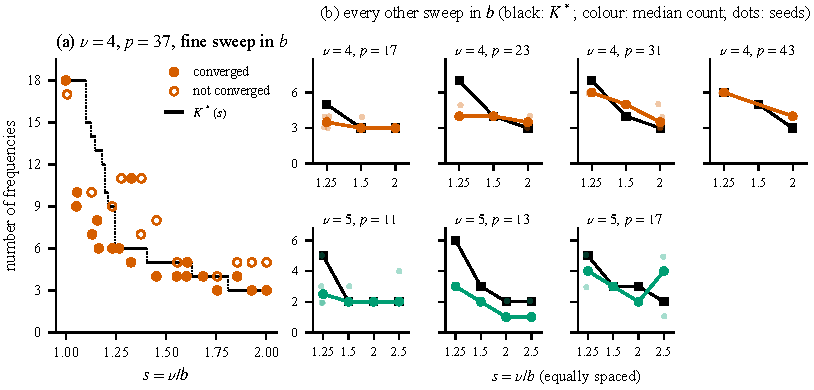
\includegraphics[width=\linewidth]{figures/fig_exponent.pdf}
\caption{\textbf{The count follows the exponent.} (a) Product networks at $\nu=4$, $p=37$, sweeping $b$ from $4$ to $2$ ($s$ from $1$ to $2$). Black: $\Kstar(s)$, exact, with its twelve plateaus (the two at $\Kstar=6$ differ in their amplitude ratios). Each marker is one run ($19$ converged, $13$ not). (b) Every other sweep in $b$ at fixed $(\nu,p)$ with at least two converged cells ($\nu=4$, $p=59$ has one and is omitted). Black: $\Kstar$; colour: median count over converged seeds; dots: individual seeds. The $s$ values are drawn equally spaced.}
\label{fig:exponent}
\end{figure}

Figure~\ref{fig:exponent}a sweeps the norm exponent at fixed degree and prime. As $b$ falls from $\nu$ to $2$, $\Kstar$ falls from $18$ (every frequency) to $3$, and the trained count falls with it: the converged run at $s=1$ uses all $18$ frequencies, and every converged run at $s\ge1.45$ is within one of $\Kstar$. Between $s=1.05$ and $1.25$, where $\Kstar$ steps through seven plateaus from $18$ to $9$, the trained counts sit below $\Kstar$ and do not resolve the plateaus: the preregistered test of the plateau identity matched in $2$ of $19$ converged runs.

Figure~\ref{fig:exponent}b shows the remaining sweeps in $b$ at $\nu=4$ and $5$; the $\nu=3$ sweeps have two values of $s$ and appear in Figure~\ref{fig:prime}. Across all of them, when $s$ changes at fixed $(\nu,p)$ the median count moves in the same direction as $\Kstar$ in $30$ of $36$ pairs, stays put in $4$ and reverses in $2$. Shuffling the counts across cells gives $38\%$ ($95$th percentile $53\%$; one-sided $p=0.001$), and on the fine grid of panel (a) the figure is $83$ of $96$ pairs against $47\%$ (post hoc). A predictor that ignores $s$ scores zero on this test. By contrast, the pooled comparison ``count within one of $\Kstar$'' holds in $70\%$ of converged runs but already in $50\%$ for the best constant, so it discriminates little. The counts move about half as far as $\Kstar$ (slope $0.50$; $0.27$--$0.61$ across count definitions and the two sweeps).

\begin{figure}[t]
\centering
\includegraphics[width=\linewidth]{figures/fig_spectra.pdf}
\caption{\textbf{From dense to sparse at $\nu=3$.} Fourier amplitudes $A_j/\max_kA_k$ of one converged product network per panel (chosen by rule: the lowest converged seed). Coloured bars pass the counting threshold (dotted, $0.2$); grey bars do not. Top: $b=\nu=3$, where Corollary~\ref{cor:dense} predicts every frequency with equal amplitude. Middle and bottom: $b=2.4$ and $b=2$.}
\label{fig:spectra}
\end{figure}

At the dense end, $b=\nu$ (Figure~\ref{fig:spectra}), trained product networks are dense and near-flat at $\nu=3$ ($p=23,59,113$: smallest amplitude at least $0.55$ of the largest, total variation to uniform at most $0.034$) and at $\nu=4$, $p=23$, as is the power network at $\nu=3$, $p=23$, and they reach $0.88$--$1.00$ of the ceiling. At $\nu=5$ converged runs are dense but not flat (total variation to uniform $0.10$--$0.41$), and at $\nu=4$, $p\ge43$ and for the power network at $p\ge59$ no run converged. Density alone is not diagnostic, since at initialization all but at most two frequencies already exceed $10\%$ of the largest amplitude; flatness is.

\subsection{Moving the degree and the norm separately}

Theorem~\ref{thm:cyclic} says that $\nu$ and $b$ enter only through $s$. Two post-hoc tests on the main sweep probe this, and neither is conclusive at a few seeds per cell. At fixed $b=2$ (weight decay), raising $\nu$ raises $s$ and lowers $\Kstar$ (Table~\ref{tab:kstar}); the median count moves the same way in $5$ of $7$ pairs, with one tie and one reversal ($p=0.16$; $3$ to $7$ of $7$ across count definitions). At fixed $s$, $\Kstar$ does not depend on $\nu$, yet the median counts of cells with the same $(p,s)$ and different $\nu$ differ by $1.1$ on average, against $1.3$ between cells with the same $\nu$ and different $s$ (where $\Kstar$ differs by $2.3$). The data are therefore consistent with the degree mattering through $s$ at weight decay, but they do not establish that $s$ alone decides the count.

\begin{figure}[t]
\centering
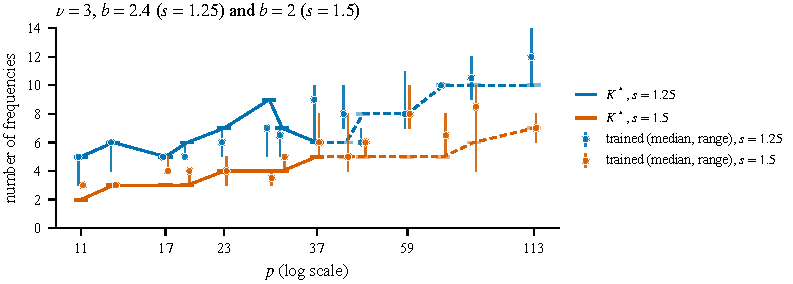
\includegraphics[width=\linewidth]{figures/fig_prime.pdf}
\caption{\textbf{The count across primes}, product networks at $\nu=3$. Lines: $\Kstar$ (solid where exact, $p\le37$; dashed where best found). Markers: median over converged seeds, with the range. $\Kstar$ is not monotone in $p$ (at $s=1.25$ it is $9,7,6$ at $p=29,31,37$); the trained counts do not follow these steps.}
\label{fig:prime}
\end{figure}

Across primes (Figure~\ref{fig:prime}), the median count is within one of $\Kstar$ in $20$ of $28$ $(p,s)$ cells up to $p=113$, against $16$ for the best constant at each $s$ (post hoc). It does not follow the non-monotone steps of $\Kstar$ in $p$, and at $s=1.5$ and $p\ge59$ it exceeds $\Kstar$ by one to three. Logarithmic growth cannot be tested over this range of $p$.
